%! TeX root = master.tex
% !TEX program = lualatex
\lecture{12}{12-05-2026}{Clustering}{}

\section{Clustering: another unsupervised task}
Dimensionality reduction transformed the data into a lower-dimensional representation.
\textbf{Clustering} is a different unsupervised task: given a set of input samples, we want
to identify natural \textbf{groups} of similar samples \emph{without} performing any data
transformation. The output is therefore not a new representation but a \textbf{partition} of
the data into clusters.

\begin{center}
  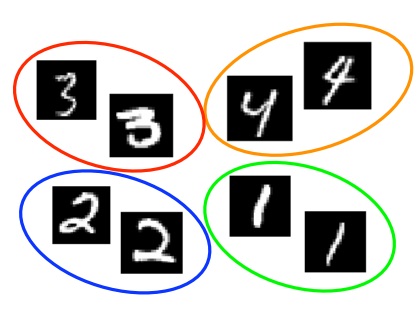
\includegraphics[width=0.3\linewidth]{images/img_20260512_134521.png}
\end{center}

A typical motivating example is grouping human poses observed in a collection of paintings
(Impett \& S\"usstrunk, 2017), so as to discover recurring poses across different artists. Each
sample is then a high-dimensional pose vector, and clustering yields a small number of
prototypical poses.

\begin{center}
  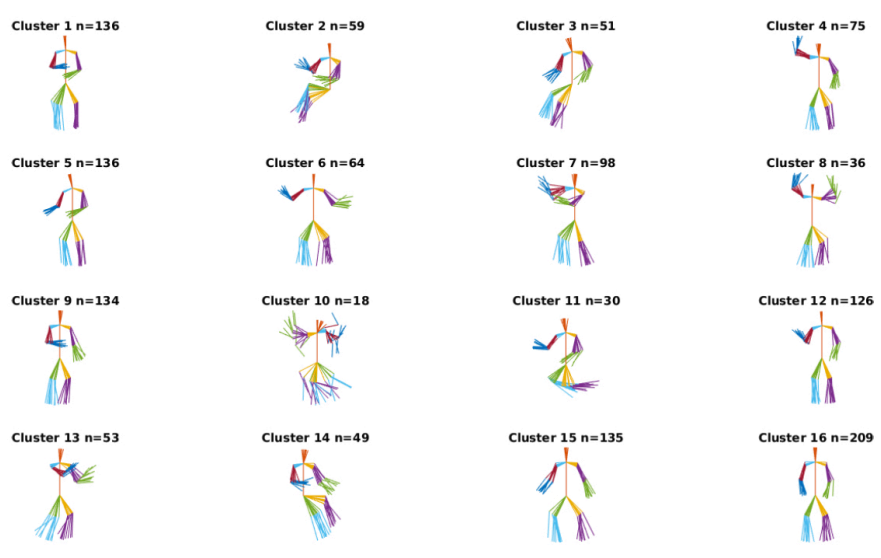
\includegraphics[width=0.9\linewidth]{images/img_20260512_134706.png}
\end{center}

Another classical use is the construction of a \textbf{visual dictionary}: image patches are
grouped by similarity, and the center of each group becomes a ``visual word''.

\section{K-means clustering}
\subsection{Intuition}
K-means is the simplest clustering algorithm. The user specifies a number of clusters $K$
(a \textbf{hyper-parameter}, assumed given) and the algorithm groups the $N$ samples into
$K$ clusters such that:
\begin{itemize}
  \item the distances between points \emph{within} the same cluster are small,
  \item the distances \emph{across} clusters are large.
\end{itemize}
This is encoded via $K$ \textbf{cluster centers} $\{\mu_1, \dots, \mu_K\}$: each sample is
assigned to the nearest center, and the centers themselves are placed at the mean of their
assigned samples.

\paragraph{Example}
For samples that act as a 2D points
\begin{center}
  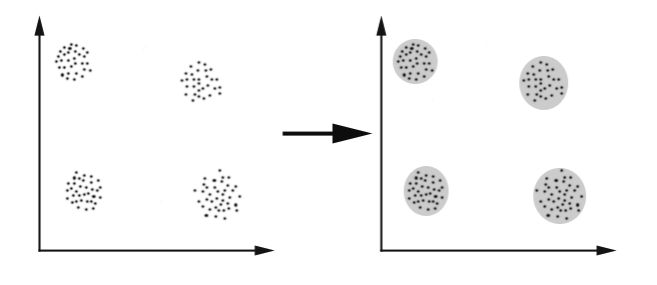
\includegraphics[width=0.6\linewidth]{images/img_20260512_135522.png}
\end{center}

\subsection{Algorithm}
The algorithm alternates between assigning points and updating centers:
\begin{enumerate}
  \item \textbf{Initialize} the centers $\{\mu_1, \dots, \mu_K\}$ (e.g, randomly).
  \item \textbf{While not converged}:
  \begin{itemize}
    \item \textbf{Assignment step}: for each point $x_i$, compute the Euclidean distance to every center $\mu_k$, and assign $x_i$ to the cluster with the smallest distance. Each point belongs to a single cluster.
    \item \textbf{Update step}: recompute each center $\mu_k$ as the \emph{mean} of the points currently assigned to it.
  \end{itemize}
\end{enumerate}

\subsubsection{Convergence}
The algorithm iteratively updates assignments and centers. We need a stopping criterion.
Using a fixed number of iterations is arbitrary and dangerous if too small. A better criterion
is to stop when the assignments (or the centers) no longer change between two iterations:
\textbf{K-means is guaranteed to converge} to such a stable solution.

\textbf{Important caveat:} convergence does not mean optimality. The solution reached depends
heavily on the \textbf{initialization} of the centers, and different initializations can lead
to different (sometimes much worse) clusterings.

\subsection{Properties and practical considerations}
\textbf{Pros:}
\begin{itemize}
  \item Simple algorithm, guaranteed to converge.
  \item Returns exactly $K$ clusters.
  \item Fully unsupervised: only needs the data, no labels. 
  \item The Euclidean distance works well when all dimensions are \emph{homogeneous}.
\end{itemize}

\textbf{Cons and remedies:}
\begin{itemize}
  \item \textbf{May converge to a bad local optimum.} Run the algorithm several times with
        different initializations; for each run, compute the sum of distances from points to
        their assigned center; keep the run with the smallest sum.
  \item \textbf{Some clusters may end up empty} (no point assigned).
  \item \textbf{The user must choose $K$.} Since clustering is unsupervised,
        cross-validation is not an option. A common heuristic is the \textbf{elbow method}
        described below.
      \item \textbf{The dimensions may be heterogenous} thus the euclidian distance will works poorly. Normalize the data or use a different distance function.
\end{itemize}

If class labels happen to be available afterwards, they can be used to \emph{label} each
cluster: for each cluster, count the number of samples of each category and assign the cluster
the majority category. Without labels, providing a semantic meaning to a cluster requires
human inspection of its members.

\subsubsection{Elbow method for choosing $K$}
Run K-means for increasing values of $K$ and plot the average within-cluster distance (sum of
squared distances from points to their assigned center) as a function of $K$. This curve
typically decreases towards $0$ (the extreme being one cluster per point). The
\textbf{``elbow''} is the value of $K$ beyond which the gain in within-cluster distance
becomes marginal: it offers a reasonable trade-off between cluster compactness and
interpretability.

\begin{center}
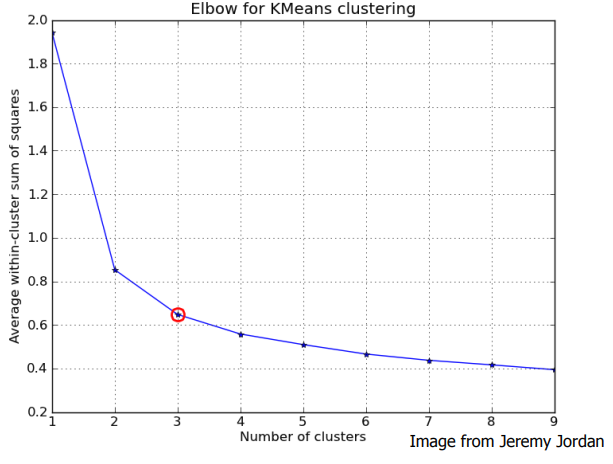
\includegraphics[width=0.7\linewidth]{images/img_20260512_140845.png}
\end{center}

\subsection{Example: color-based image segmentation}
A natural application of K-means is image segmentation by color: each pixel
is treated as a data point $x_i \in \mathbb{R}^3$ encoded by its RGB values, and K-means
groups pixels with similar colors. Increasing $K$ yields finer segmentations.

\begin{center}
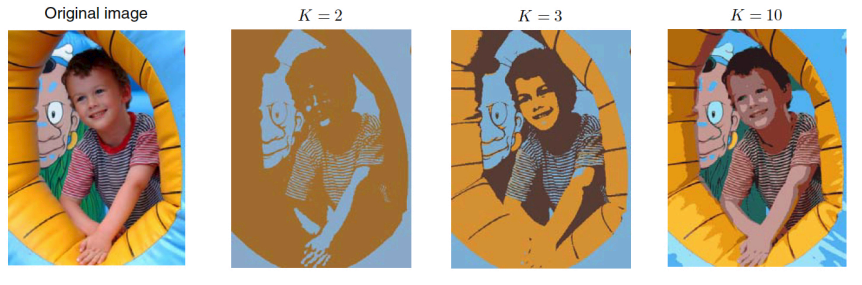
\includegraphics[width=\linewidth]{images/img_20260512_140413.png}
\end{center}

\subsection{The Euclidean distance is not always appropriate}
The Euclidean distance works well when all dimensions are \emph{homogeneous} (commensurate
magnitudes, comparable semantics). This was the case in the previous examples: 2D toy points,
RGB pixels in $[0,255]^3$, or human pose vectors where every dimension represents the same
type of quantity.

In practice this is not always the case. Different dimensions can have wildly different
magnitudes \emph{and} represent completely different kinds of information.

\textbf{Example } Consider the
\textbf{Wine dataset} (UCI ML repository): 178 wines from 3 producers, each described by 13
attributes such as alcohol content, malic acid, magnesium. Two samples:
\[
\begin{array}{l}
\text{Sample 1: } [14.37,\; 1.95,\; 2.5,\; 16.8,\; 113,\; 3.85,\; 3.49,\; 0.24,\; 2.18,\; 7.8,\; 0.86,\; 3.45,\; 1480] \\
\text{Sample 2: } [13.24,\; 2.59,\; 2.87,\; 21,\; 118,\; 2.8,\; 2.69,\; 0.39,\; 1.82,\; 4.32,\; 1.04,\; 2.93,\; 735]
\end{array}
\]
The last dimension (proline content, in the thousands) will dominate the Euclidean distance
and crush the contribution of all other features -- although there is no reason to think it
is more meaningful for the clustering.

\textbf{Solution:} \emph{normalize} (e.g, scale each dimension to zero mean and unit variance)
and/or use a different distance function. On the wine data this makes a large difference:

\begin{center}
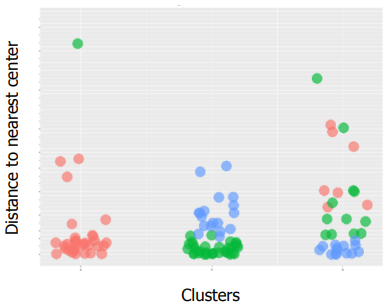
\includegraphics[width=0.305\linewidth]{images/img_20260512_141805.png}
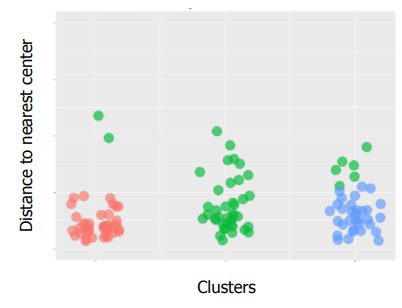
\includegraphics[width=0.32\linewidth]{images/img_20260512_141823.png}
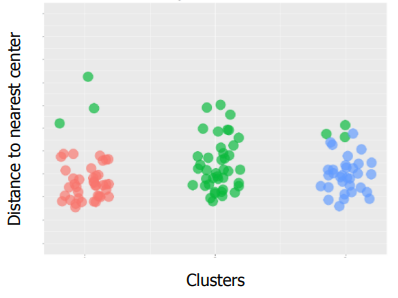
\includegraphics[width=0.32\linewidth]{images/img_20260512_141833.png}
\end{center}
\begin{itemize}
  \item Fig. 1: Euclidean distance, raw data: $70.3\%$ accuracy. 
  \item Fig. 2: Euclidean distance, scaled data: $93.2\%$ accuracy.
  \item Fig. 3: $L^1$ distance, scaled data: $94.5\%$ accuracy.
\end{itemize}
(Here \emph{accuracy} means the percentage of samples assigned to the correct cluster, after
matching each cluster to its majority producer.)


\section{Fisher Linear Discriminant Analysis (LDA)}
The dimensionality reduction methods we saw last week (PCA, kernel PCA, autoencoders) are
\textbf{unsupervised}. As a result, they may project the data in directions that mix up
classes -- nothing tells PCA that some directions are more semantically meaningful than
others.

\begin{center}
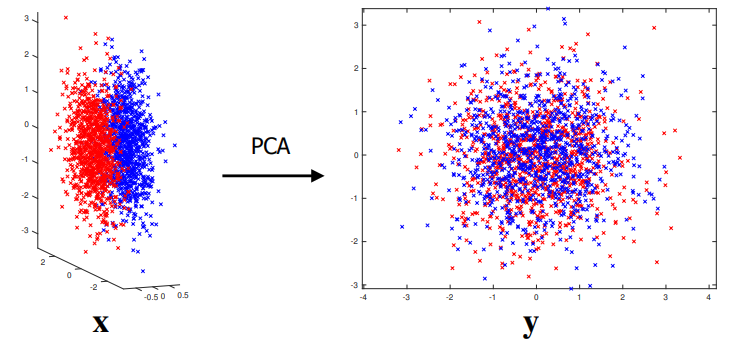
\includegraphics[width=0.6\linewidth]{images/img_20260512_142424.png}
\end{center}

If class labels \emph{are} available, we can do better. \textbf{Fisher LDA}
combines clustering and dimensionality reduction by looking for a projection in which
\begin{itemize}
  \item samples from the \emph{same} class cluster tightly,
  \item different classes are well \emph{separated}.
\end{itemize}
Note that we are technically back to supervised learning, but the supervision is not used to
predict $\{y_i\}$ directly: it only guides the projection. The intuition is the same as
K-means -- small within-cluster spread, large between-cluster spread -- but applied
\emph{after} a linear projection.

\subsection{Clustering within each class: within-class scatter}
Consider a 1D projection given by a vector $w_{(1)} \in \mathbb{R}^D$, and $C$ classes. Let
$y_i = w_{(1)}^T x_i$ and let $\nu_c$ be the mean of the projections of class $c$. To cluster
the samples of each class, we want \textbf{low variance within each class after projection},
i.e, minimize
\[
E_W(w_{(1)}) = \sum_{c=1}^{C} \sum_{i \in c} (y_i - \nu_c)^2,
\]
where $\nu_c$ is the mean of the samples in class $c$ after projection, and $i \in c$ means ``sample $i$ belongs to class $c$''. Both $y_i$ and $\nu_c$ depend on
$w_{(1)}$.

Since the projection is linear, the class-mean after projection is the projection
of the class-mean before projection:
\[
\nu_c = \frac{1}{N_c} \sum_{i \in c} y_i = \frac{1}{N_c} \sum_{i \in c} w_{(1)}^T x_i = w_{(1)}^T \mu_c,
\qquad \text{so} \qquad
y_i - \nu_c = w_{(1)}^T (x_i - \mu_c),
\]
where $\mu_c$ is the mean of class $c$ before projection.

As we did for PCA, the variance after projection equals the projection of a covariance-like
matrix, which lets us rewrite this as
\[
E_W(w_{(1)}) = w_{(1)}^T S_W \, w_{(1)},
\qquad
S_W = \sum_{c=1}^{C} \sum_{i \in c} (x_i - \mu_c)(x_i - \mu_c)^T,
\]
where $\mu_c$ is the mean of class $c$ \emph{before} projection. The matrix $S_W$ is called
the \textbf{within-class scatter matrix}.

\subsection{Separating the classes: between-class scatter}
To separate clusters, we also want to push the class means \emph{away} from each other after
projection. Letting $\bar{y}$ denote the mean of all projected samples and $N_c$ the number
of samples in class $c$, we want to \emph{maximize}
\[
E_B(w_{(1)}) = \sum_{c=1}^{C} N_c (\nu_c - \bar{y})^2.
\]
By the same reasoning,
\[
E_B(w_{(1)}) = w_{(1)}^T S_B \, w_{(1)},
\qquad
S_B = \sum_{c=1}^{C} N_c \,(\mu_c - \bar{x})(\mu_c - \bar{x})^T,
\]
where $\bar{x}$ is the mean of all samples. $S_B$ is called the \textbf{between-class scatter
matrix}.

\subsection{Fisher LDA objective}
We want simultaneously to:
\begin{itemize}
  \item \textbf{Minimize} $E_W(w_{(1)})$ (tight classes),
  \item \textbf{Maximize} $E_B(w_{(1)})$ (well-separated classes).
\end{itemize}
A standard trick to do both at once is to maximize their \emph{ratio}: minimizing $f(\cdot)$
is, in general, achieved by maximizing $1/f(\cdot)$. We therefore maximize
\[
J(w_{(1)}) = \frac{E_B(w_{(1)})}{E_W(w_{(1)})}
           = \frac{w_{(1)}^T S_B \, w_{(1)}}{w_{(1)}^T S_W \, w_{(1)}}.
\]

\subsubsection{Scaling invariance and the constrained form}
$J$ is invariant to the scaling of $w_{(1)}$, i.e, $J(\alpha w_{(1)}) = J(w_{(1)})$ for any
$\alpha \in \mathbb{R}$. We can therefore fix the scale by imposing $w_{(1)}^T S_W \, w_{(1)} = 1$,
giving the Fisher LDA formulation
\[
\max_{w_{(1)}} w_{(1)}^T S_B \, w_{(1)} \quad \text{s.t.} \quad w_{(1)}^T S_W \, w_{(1)} = 1.
\]

\subsubsection{Generalized eigenvalue problem}
Forming the Lagrangian
\[
\mathcal{L}(w_{(1)}, \lambda_1) = w_{(1)}^T S_B \, w_{(1)} + \lambda_1 \bigl(1 - w_{(1)}^T S_W \, w_{(1)}\bigr)
\]
and setting its gradient w.r.t. $w_{(1)}$ to zero yields
\[
\boxed{\, S_B \, w_{(1)} = \lambda_1 S_W \, w_{(1)} \,}
\]
which is a \textbf{generalized eigenvalue problem}. Left-multiplying by $w_{(1)}^T$ and dividing
by $w_{(1)}^T S_W \, w_{(1)} = 1$ shows that the value of the objective $J$ at the optimum is
exactly $\lambda_1$, so we should pick the eigenvector $(w_{(1)})$ with the \textbf{largest eigenvalue}.

\subsubsection{From 1D to $d$-dimensional projections}
As for PCA, more output dimensions are obtained recursively: take the $d$ eigenvectors of the
generalized problem with the largest eigenvalues.

\textbf{An important limitation:} the rank of $S_B$ is at most $C - 1$ (it is a sum of $C$ rank-1
matrices that are linearly dependent through the constraint that all class means average to
$\bar{x}$). The remaining eigenvalues are exactly zero, so Fisher LDA can only project the
data to at most $C - 1$ dimensions. With 10 MNIST digit classes, this caps us at 9 LDA
directions.

\subsection{Example: visualizing MNIST}
Projecting MNIST digits with Fisher LDA:

\begin{center}
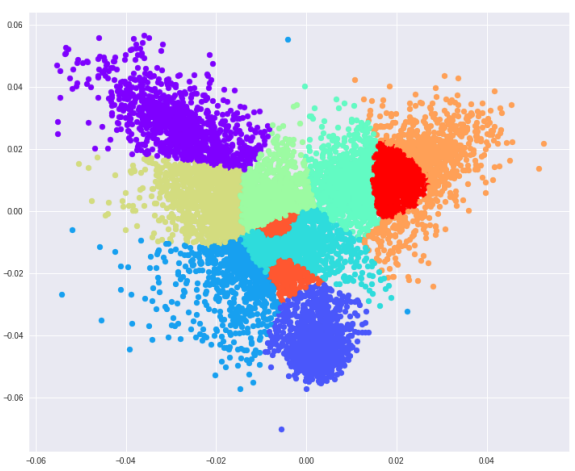
\includegraphics[width=0.4\linewidth]{images/img_20260512_153736.png}
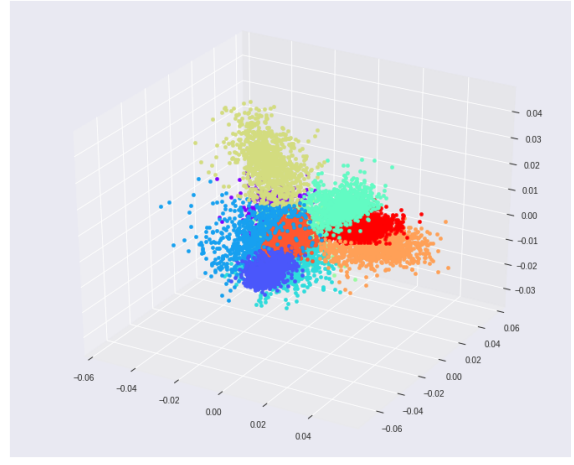
\includegraphics[width=0.4\linewidth]{images/img_20260512_153758.png}
\end{center}

\begin{itemize}
  \item in 2D, the classes form somewhat separated blobs, classification accuracy in the LDA space: $56\%$.
  \item in 3D, the separation improves significantly, classification accuracy: $74\%$.
\end{itemize}

\subsection{Eigenfaces vs Fisherfaces}
Consider a face dataset with 2 expressions (treated as 2 classes) and several illumination
conditions. Applying PCA or Fisher LDA to vectorized face images yields eigenvectors that can
themselves be visualized as images:
\begin{itemize}
  \item the PCA directions are called \textbf{eigenfaces},
  \item the LDA directions are called \textbf{fisherfaces}.
\end{itemize}
\begin{center}
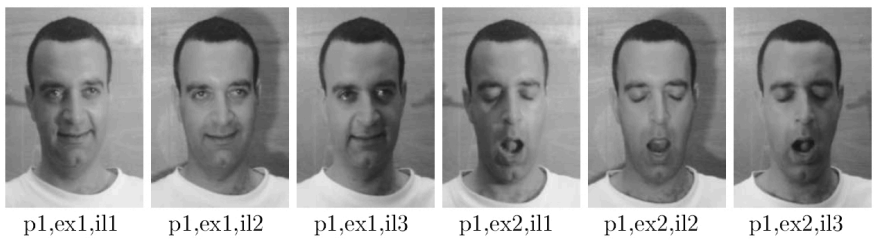
\includegraphics[width=\linewidth]{images/img_20260512_155547.png}
\end{center}
\clearpage
\textbf{Eigenfaces} minimize the reconstruction error. They therefore must capture whatever
explains most of the variance in the data -- and illumination changes induce huge pixel
variations. Eigenfaces end up encoding a lot of illumination information.
\begin{center}
  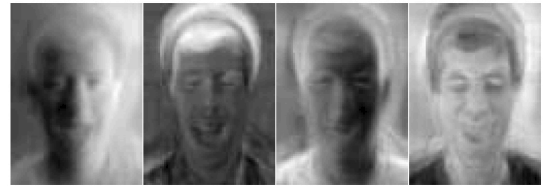
\includegraphics[width=0.5\linewidth]{images/img_20260512_160100.png}
\end{center}
Image reconstruction: 
\begin{center}  
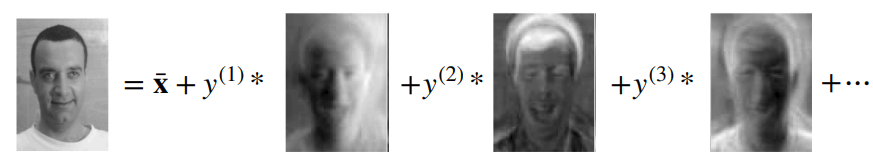
\includegraphics[width=\linewidth]{images/img_20260512_160238.png}
\end{center}

\textbf{Fisherfaces} are explicitly chosen to be discriminative of the class (here:
expression). They therefore \emph{discard} illumination, which is irrelevant to expression
recognition, and emphasize features around the mouth and eyes.
\begin{center}
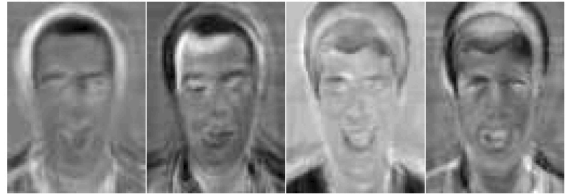
\includegraphics[width=0.5\linewidth]{images/img_20260512_160548.png}
\end{center}

This is a nice illustration of how the choice of objective dictates which features survive
projection: \emph{maximum variance} (PCA) and \emph{maximum discriminability} (LDA) can lead
to very different bases.

\section{Spectral clustering}
\subsection{Why K-means and LDA can fail}
K-means and Fisher LDA both rely on the notion of \textbf{compactness}: each cluster is
expected to be a tight blob around its mean. This works well on data with compact samples
but fails on data that is not compact. The classical pathological case is \textbf{two
concentric circles}: there are clearly two natural clusters, but K-means -- which only sees
distances to centers -- cuts the data in half through the middle.
\begin{center}
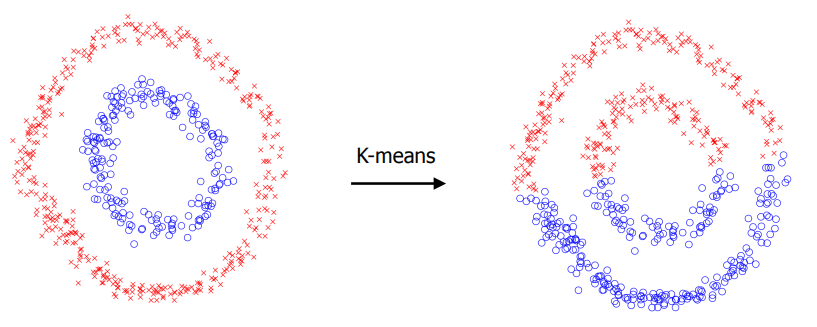
\includegraphics[width=0.6\linewidth]{images/img_20260512_160953.png}
\end{center}

\subsection{Connectivity as the right notion}
What separates the two circles is \textbf{connectivity}: every point on the inner circle has
close neighbors that are themselves on the inner circle, and similarly for the outer circle,
while no inner-circle point is close to any outer-circle point. We can model this with a
\textbf{graph} whose nodes are the data points and whose edges encode local similarity (strong connections indicates nodes that should be clustered, weaker ones suggests that the graph can be cut into pieces/partitions).
\begin{center}
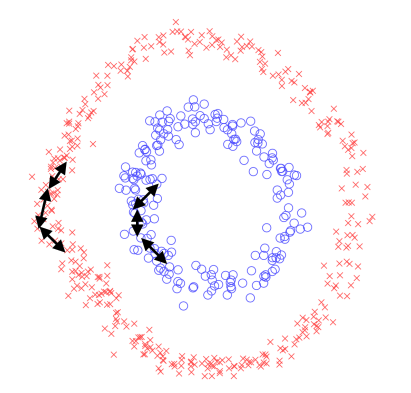
\includegraphics[width=0.2\linewidth]{images/img_20260512_162533.png}
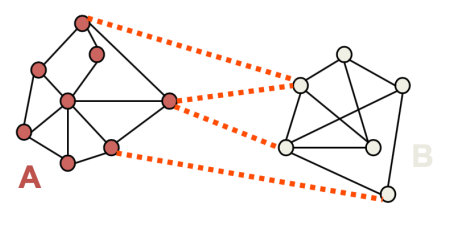
\includegraphics[width=0.4\linewidth]{images/img_20260512_162629.png}
\end{center}

\subsection{Building the graph}
The similarity (connectivity) between points $i$ and $j$ is typically encoded by a positive weight $W_{ij}$.
A standard choice is the Gaussian (RBF) similarity
\[
W_{ij} = \exp\!\left( \frac{-\|x_i - x_j\|^2}{\sigma^2} \right),
\]
where $\sigma$ is a hyper-parameter controlling how quickly similarity decays with distance.
This yields a \textbf{fully-connected} graph (every pair of points has an edge), but one
typically restricts the graph to the \textbf{$K$-nearest neighbors} of each point to encode
locality and keep the graph sparse.

A graph is equivalently described by its \textbf{similarity (affinity) matrix} $W \in \mathbb{R}^{N \times N}$.
\begin{center}
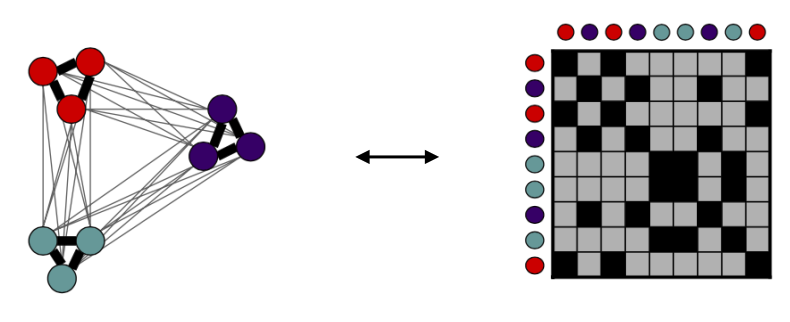
\includegraphics[width=0.5\linewidth]{images/img_20260512_163351.png}
\end{center}

\subsection{Graph cut}
Consider a partition of the graph into two sets $A$ and $B$. The \textbf{cut} between $A$ and
$B$ is the total weight of the edges that connect them:
\[
\mathrm{cut}(A, B) = \sum_{i \in A, j \in B} W_{ij}.
\]
Intuitively, a good clustering minimizes the cut: we want few, weak edges across the
boundary.

\begin{center}
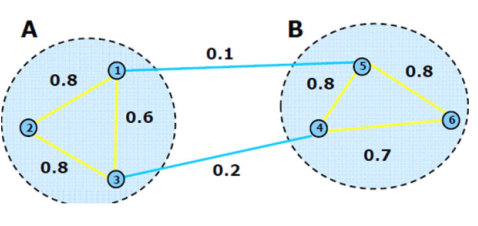
\includegraphics[width=0.5\linewidth]{images/img_20260512_163646.png}
\end{center}

\subsection{Graph terminology}
We will also need:
\begin{itemize}
  \item The \textbf{degree} of a node: $d_i = \sum_{j} W_{ij}$ (total weight incident on $i$).
    \begin{center}
      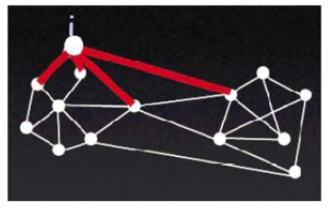
\includegraphics[width=0.25\linewidth]{images/img_20260512_164006.png}
      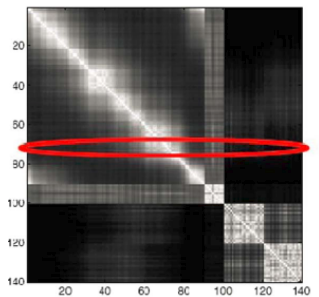
\includegraphics[width=0.25\linewidth]{images/img_20260512_164013.png}
    \end{center}     
  \item The \textbf{volume} of a set: $\mathrm{vol}(A) = \sum_{i \in A} d_i$ (total degree of nodes in $A$).
    \begin{center}
      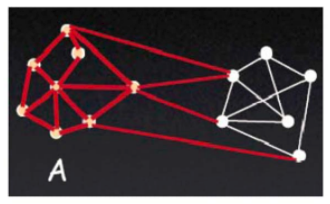
\includegraphics[width=0.25\linewidth]{images/img_20260512_163944.png}
      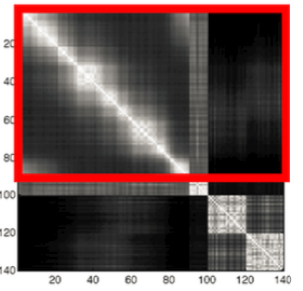
\includegraphics[width=0.25\linewidth]{images/img_20260512_163953.png}
    \end{center}
\end{itemize}

\subsection{Normalized cut}
Minimizing $\mathrm{cut}(A,B)$ alone is misleading: cutting a single isolated point off as
``cluster $A$'' often gives a very small cut while being a useless clustering. To prevent
this, we use the \textbf{normalized cut}, which penalizes imbalanced partitions by dividing
by the volume of each side:
\[
\mathrm{Ncut}(A, B) = \frac{\mathrm{cut}(A, B)}{\mathrm{vol}(A)} + \frac{\mathrm{cut}(A, B)}{\mathrm{vol}(B)}.
\]
If $A$ contains only a tiny fraction of the graph, its volume is small ($\geq cut(A,B)$) and the first term
could be close to $1$. As $\frac{\mathrm{cut}(A, B)}{\mathrm{vol}(A)} \in [0, 1]$ a balanced partition is preferred.

\subsection{Transformed formulation}
Finding the partition that minimizes $\mathrm{Ncut}$ is \textbf{NP-hard} (we are choosing one
of $2^N$ partitions). It can however be rewritten as the optimization problem
\[
\min_{y} \; \frac{y^T (D - W) y}{y^T D y}
\quad \text{s.t.} \quad
y^T D \mathbf{1} = 0,\;\;
y_i \in \{1, -b\} \;\;\forall\; 1 \leq i \leq N,
\]
where:
\begin{itemize}
  \item $W \in \mathbb{R}^{N \times N}$ is the similarity matrix between all pairs of points,
  \item $D \in \mathbb{R}^{N \times N}$ is the diagonal \textbf{degree matrix} with $D_{ii} = d_i$,
  \item $y \in \mathbb{R}^N$ indicates the partition assignment of each point. 
  \item $b = \frac{vol(A)}{vol(B)}$
\end{itemize}
This is still NP-hard because of the discrete constraint $y_i \in \{1, -b\}$.

\subsection{Spectral relaxation}
The standard trick is to \textbf{relax} the discrete constraint and allow $y \in \mathbb{R}^N$:
\[
\min_{y} \; \frac{y^T (D - W) y}{y^T D y}
\quad \text{s.t.} \quad y^T D y = 1.
\]
Using the Lagrangian, this turns into the generalized eigenvalue problem
\[
\boxed{\, (D - W) \, y = \lambda \, D \, y \,}
\]
The matrix $L = D - W$ is called the \textbf{graph Laplacian}.

\subsubsection{Which eigenvector?}
The eigenvector with the \textbf{smallest} eigenvalue ($\lambda = 0$) is the trivial all-ones
vector -- it places every point in the same partition and is useless. The actual solution is
the eigenvector with the \textbf{second smallest} eigenvalue (sometimes called the
\emph{Fiedler vector}).

In an ideal case, positive entries of this eigenvector would indicate one partition and
negative entries the other. Because of the relaxation, the entries are continuous, so one has
to \textbf{threshold} them. A common choice is to threshold at the median, which yields a
balanced partition by construction.

\begin{center}
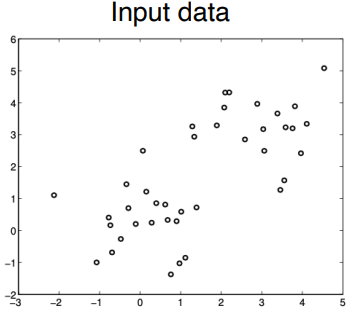
\includegraphics[width=0.3\linewidth]{images/img_20260512_194203.png}
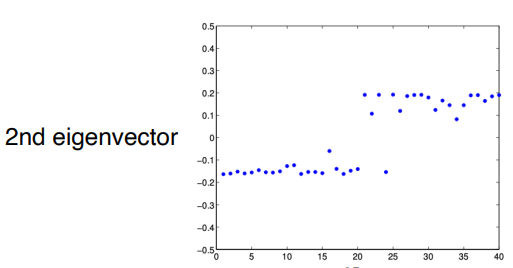
\includegraphics[width=0.5\linewidth]{images/img_20260512_193551.png}
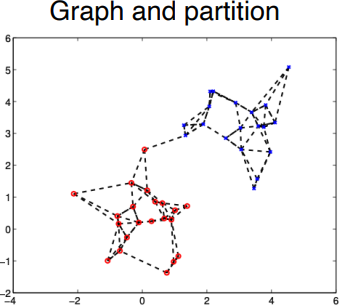
\includegraphics[width=0.3\linewidth]{images/img_20260512_194216.png}
\end{center}

\subsection{$K$-way partitioning}
To obtain more than two clusters, two strategies exist:
\begin{enumerate}
  \item \textbf{Recursive 2-way partitioning}: apply the 2-way spectral clustering, then
        recursively split each subset. This is inefficient and unstable -- small changes
        early on can propagate dramatically.
  \item \textbf{Use $K$ eigenvectors at once}: take the $K$ eigenvectors of the generalized
        problem with the smallest eigenvalues, and represent each point $i$ by the
        $K$-dimensional vector formed by stacking the $i$-th entry of each eigenvector.
        Then run \textbf{K-means} on these $K$-dimensional vectors.
\end{enumerate}
\textbf{Interpretation:} the second approach is dimensionality reduction (via the graph
Laplacian) \emph{followed by} K-means. Spectral clustering can therefore be seen as ``K-means
on a smarter feature space'' -- one where compactness aligns with the connectivity structure
of the original data.

\paragraph{Example} with $K = 2$ and $K = 3$
\begin{center}
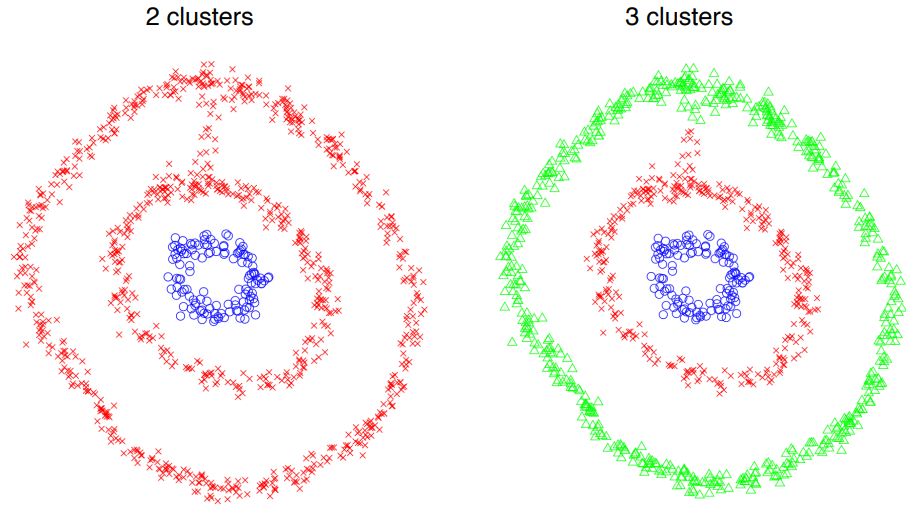
\includegraphics[width=0.6\linewidth]{images/img_20260512_194649.png}
\end{center}

\subsection{Beyond compactness and connectivity: density}
For completeness, another paradigm for clustering is \textbf{density-based} clustering
(e.g, DBSCAN), which defines clusters as regions of high point density separated by regions
of low density. This is yet another way of escaping the compactness assumption of K-means.

\clearpage
